\subsection{User Interface Representation} 
As this software is to be used mostly by civil and mechanical engineers or by developers, so to make its look and feel professional, the console based user interface is designed for this software. Also shell scripting has been used for the execution of the software, which further increases its speed and is easier to use and maintain both by users and developers.\\\\
\subsection {Brief Description of Various Modules of the system}
Brief Description of Various Modules:
The various modules which have been used are as follows:\\
\textbf{Shell Scripting} -\\ 
All the modules are combined using shell scripting. The main execution is also done through scripts.\\\\
\textbf{std-flt} -\\ 
It is a one way converter which converts the file format of STAAD-PRO software i.e std to the file format of FELT software i.e flt. It uses the Flex for lexical analysis which is the first phase of Converter. It reads the input file, i.e, .std file and break down into tokens through lexical analysis. Then the tokens are parsed using Bison parser generator tool and the parsed information is used for writing the output file, i.e .flt file, which is the last phase of converter. And finally the .std file is converted to .flt file.\\\\
\textbf{flt-std} -\\
 This module completes the two way converter as it converts the file format of FELT i.e flt to the file format of STAAD-PRO, i.e std. It uses the same methodology for its conversion, i.e Lexical analysis of the input file and dividing into tokens, Parsing tokens returned after reading it and then finally Writing the output file. The Lexical analysis is done using Flex, Parsing by Bison and File is written using C++ Programming language.\\\\


\subsection{Snapshots of system with brief detail of each}
In Six Months Training, I have done Project based on Flex and Bison technology. Using this, I have done four file converter i.e. DXF Converter, GDGNE Converter, XCAD-ECAD Converter and the final project is Felt-Staad-Pro Converter.\\\\

\subsection{DXF Converter}
dxf1 - Qmake is used to compile the program. Qmake is the very first command which is used to compile this program. The make file is created by using qmake.
\begin{figure} [h!]
\centering
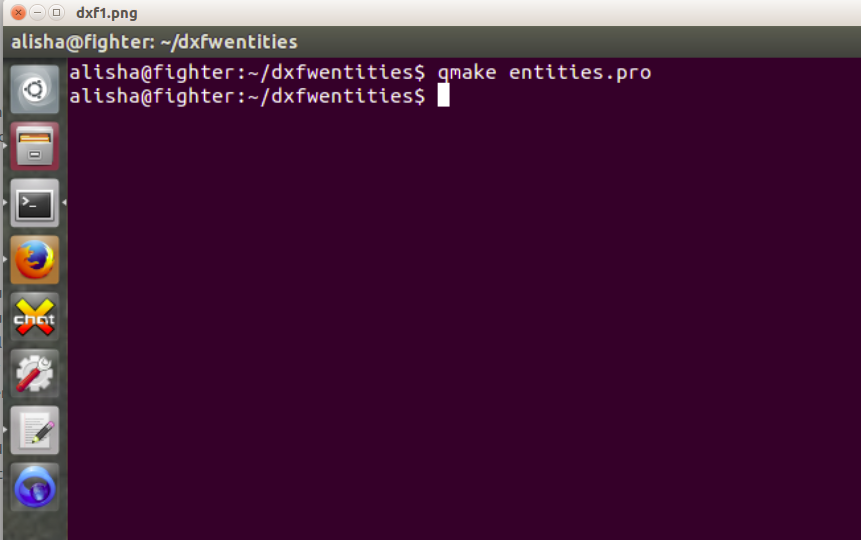
\includegraphics[scale=0.2]{images/dxf1.png}
\caption{DXF }
\end{figure}
dxf2 - The next command is make. This make command compiles the program using g++ compiler, which is a GNU compiler and used to compile programs written in C++. After this command an executable file is created, ./entities which takes input a text file and creates a dxf file based on the instructions given in the input text file.
\begin{figure} [h!]
\centering
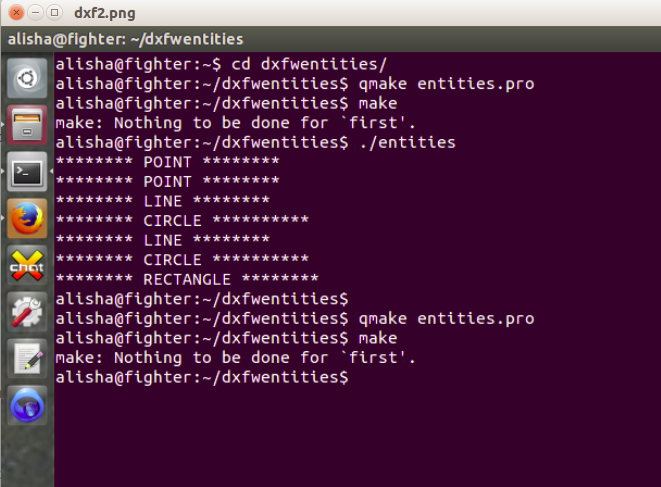
\includegraphics[scale=0.2]{images/dxf2.png}
\caption{DXF in C++ }
\end{figure}

dxf3 - The last step is to run the executable file which creates the output file i.e the dxf file. Dxf file when opened using any CAD software produces a drawing based on the instructions given in the text file and the output which is displayed on terminal which acknowledges the user, the entities which are written in dxf file.
\begin{figure} [h!]
\centering
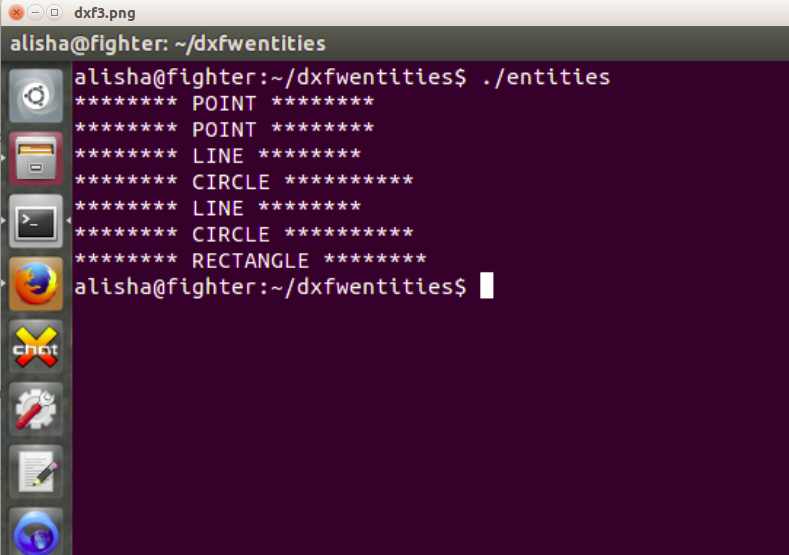
\includegraphics[scale=0.2]{images/dxf3.png}
\caption{DXF Co-ordinates}
\end{figure}

dxf4 - This is the sample input file which was given to run the program.
\begin{figure} [h!]
\centering
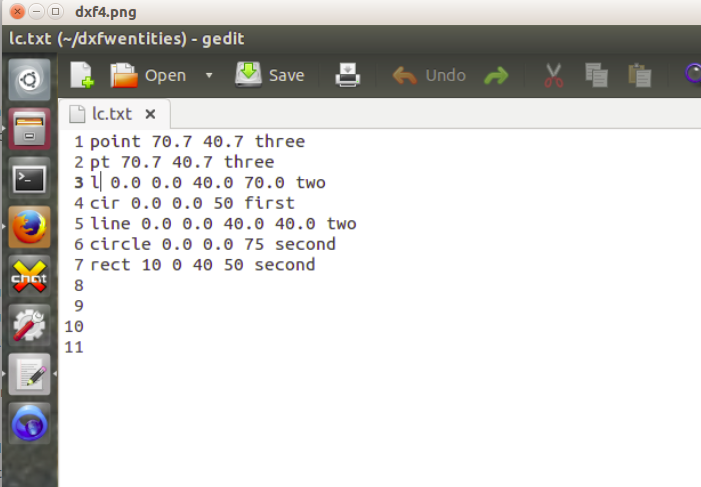
\includegraphics[scale=0.2]{images/dxf4.png}
\caption{Input File}
\end{figure}
 
dxf5 - This is the output file which produces a drawing when opened in LibreCAD, a CAD software.
\begin{figure} [h!]
\centering
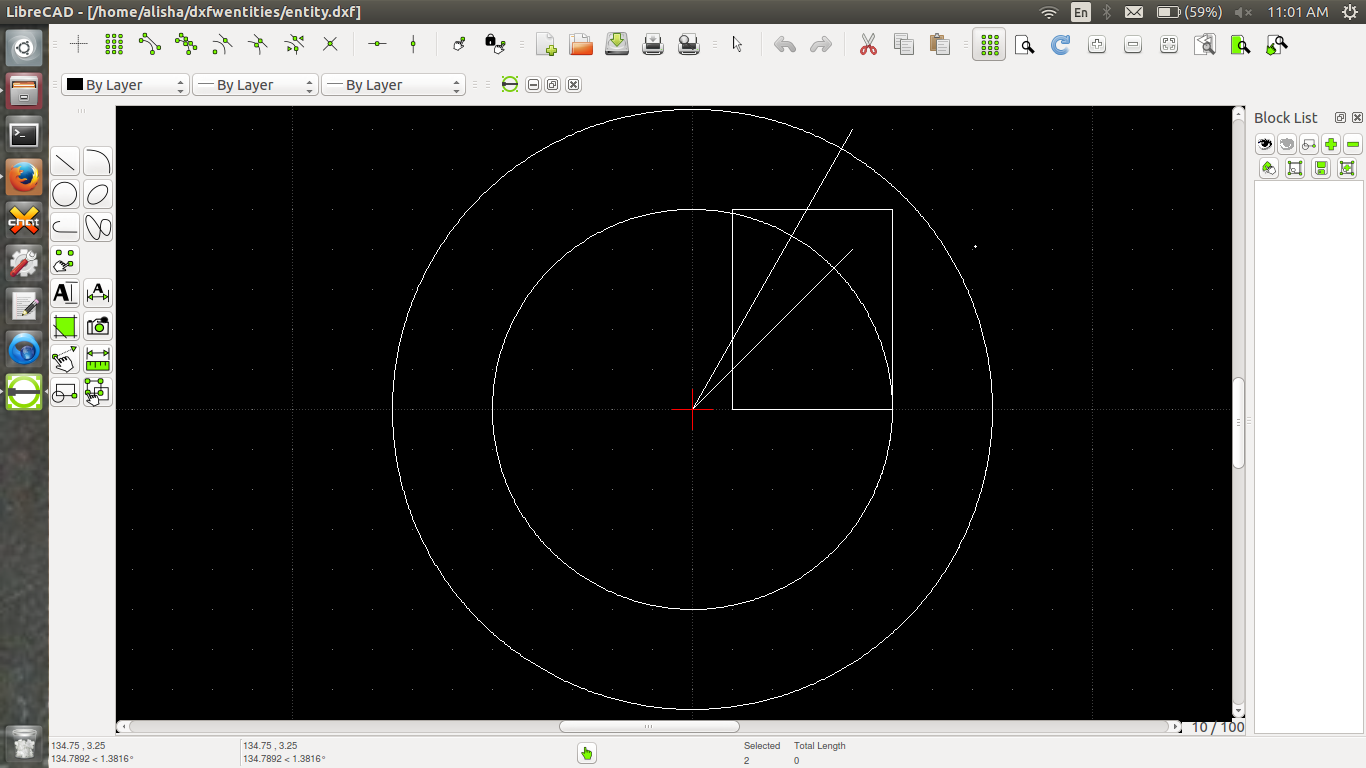
\includegraphics[scale=0.2]{images/dxf5.png}
\caption{Write DXF }
\end{figure}


\subsection{GD-GNE Converter}
GNE-GD converter is two a way converter. In which we converts on file "conv.gne" to "conv.gd". snapshots of system with brief detail of each:\\
\begin{enumerate}
\item In below figure, the list of files which we write are given. "conv.gne" and "conv.gd" are the input files. "conv.l" is lexer file and conv.y is Bison file. Parser.cc and Parser.h files are include C++ code.

\begin{figure} [h!]
\centering
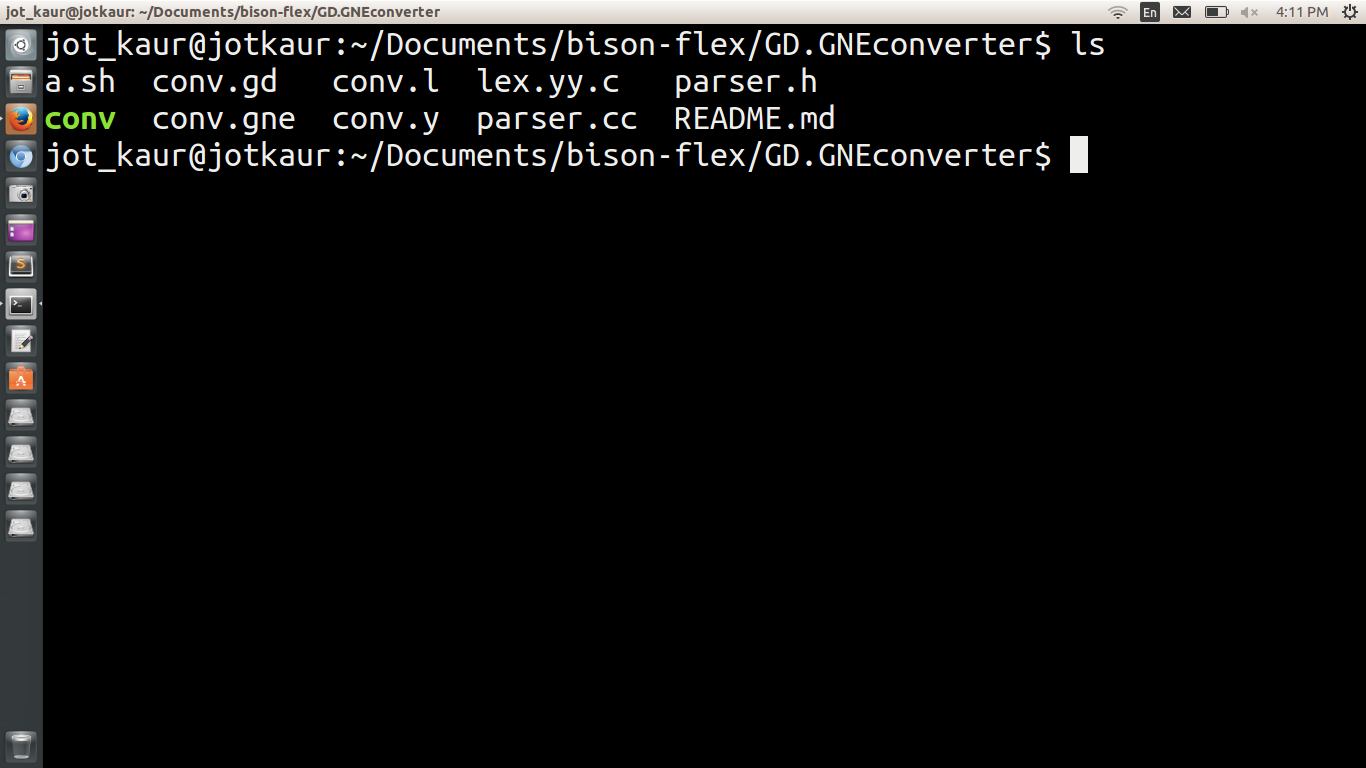
\includegraphics[scale=0.2]{images/gnefiles.png}
\caption{List Of Files  }
\end{figure}

\item Now, two library files are created by Flex and Bison. "lex.yy.c" file is generated by Flex. "conv.tab.c" and "conv.tab.h" files are generated by Bison.
\begin{figure} [h!]
\centering
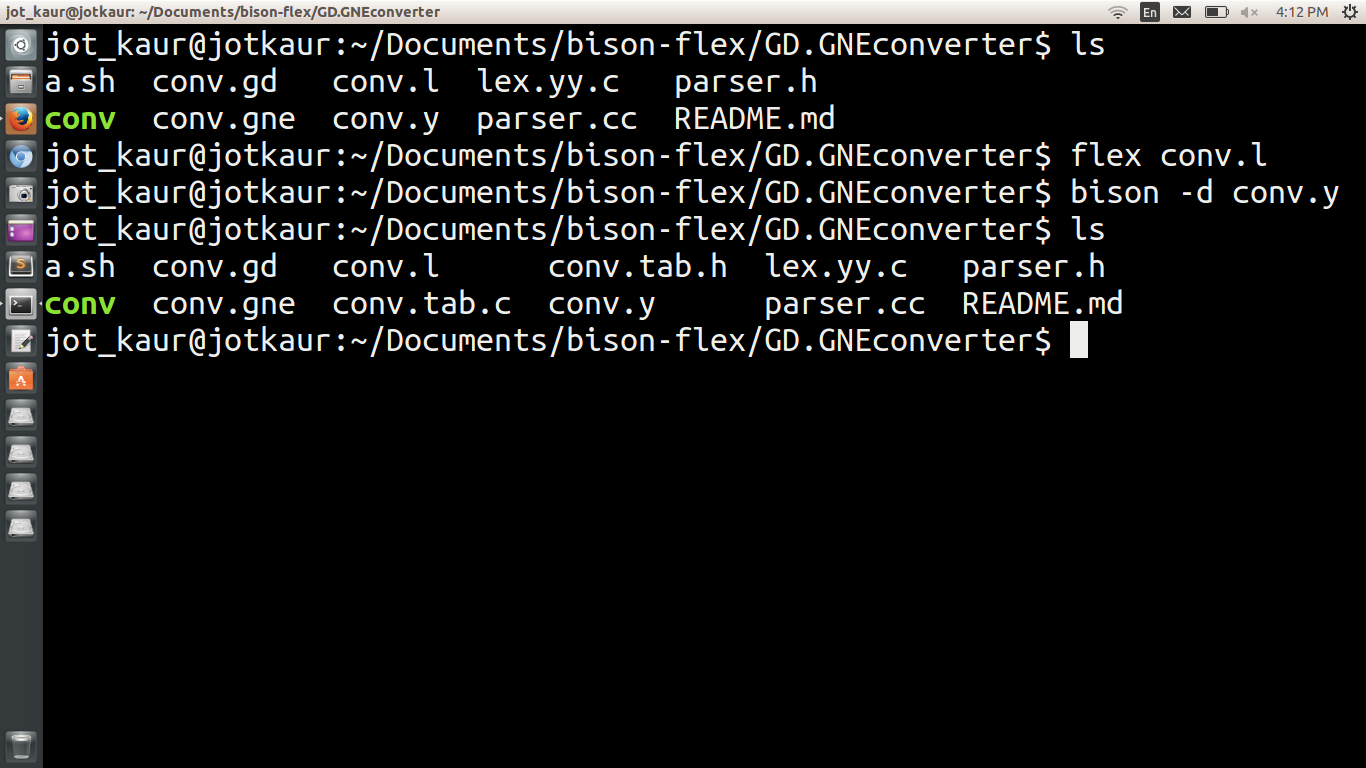
\includegraphics[scale=0.2]{images/gne2files.png}
\caption{Generate Library Files}
\end{figure}

\item "a.sh" is script which runs the code. This file includes Flex and Bison commands.
\begin{figure} [h!]
\centering
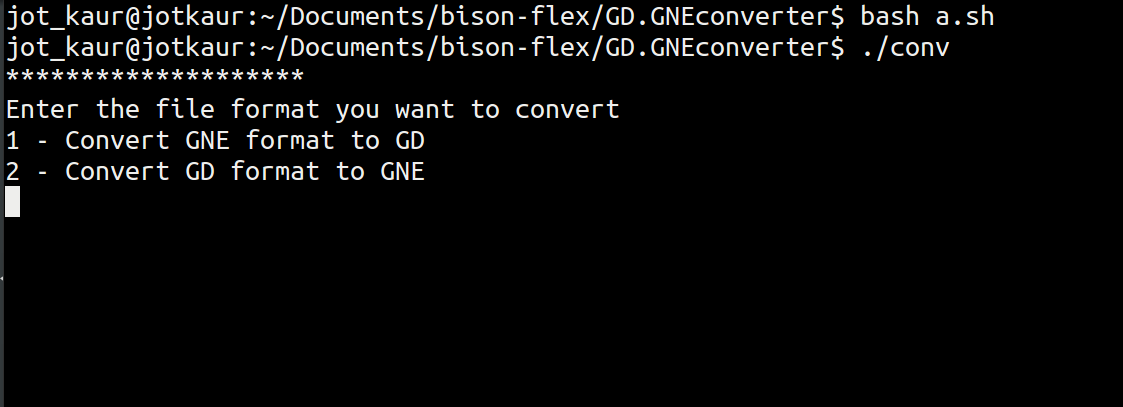
\includegraphics[scale=0.2]{images/gne1.png}
\caption{Script run}
\end{figure}

\item In screenshot the executable script shows.
\begin{figure} [h!]
\centering
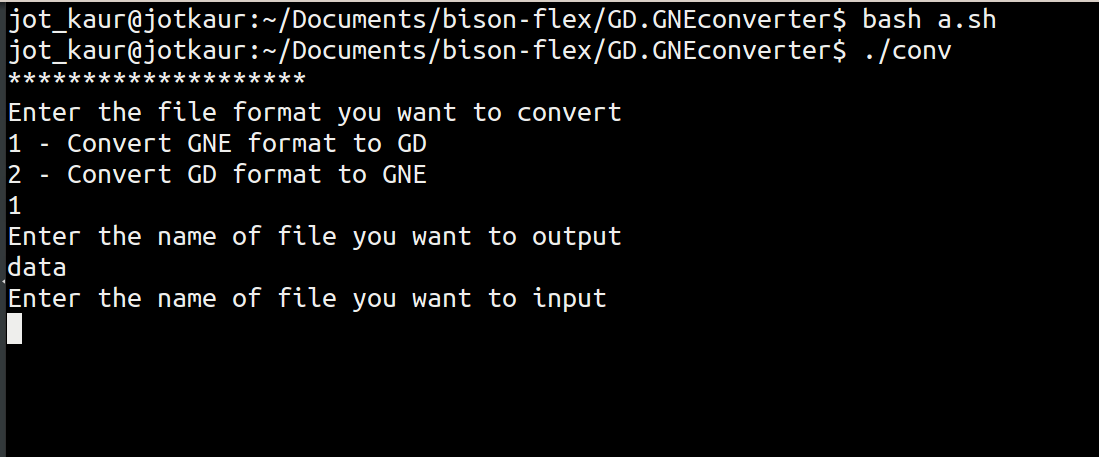
\includegraphics[scale=0.2]{images/gne2.png}
\caption{Execute script}
\end{figure}

\item As shown in image, the output file and input files are generates.
\begin{figure} [h!]
\centering
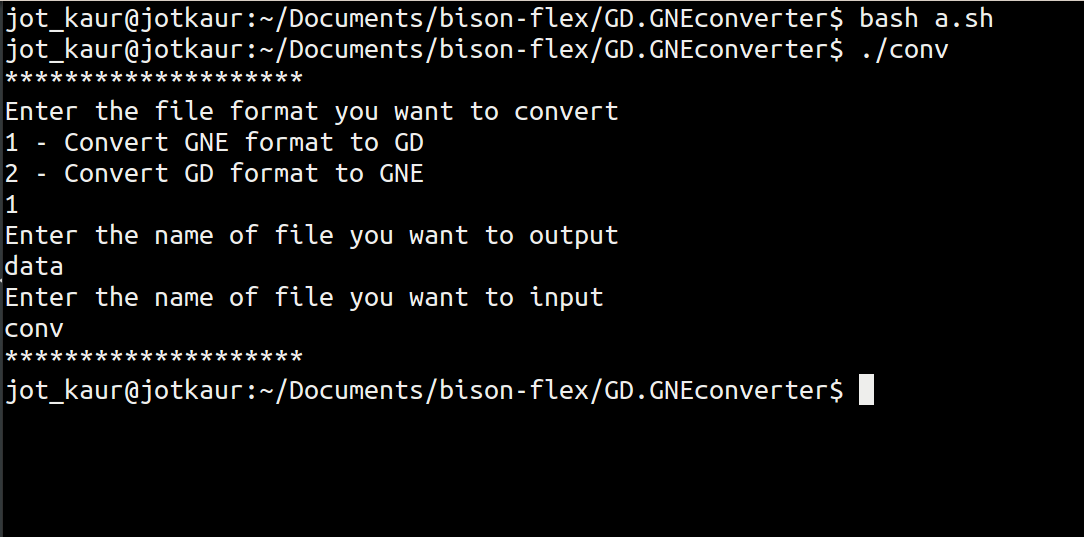
\includegraphics[scale=0.2]{images/gne3.png}
\caption{ Output File}
\end{figure}

\item Two way converter is used in GD-GNE parser which shows in image.
\begin{figure} [h!]
\centering
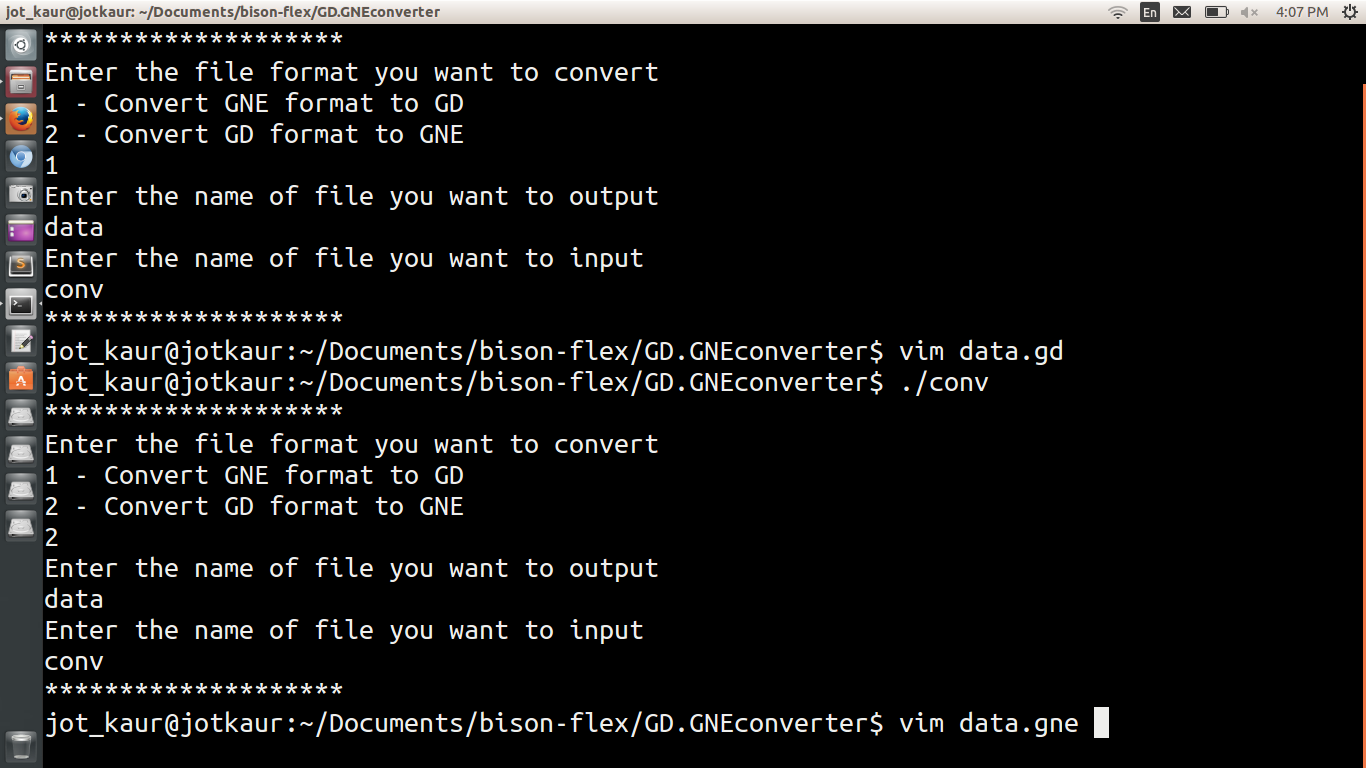
\includegraphics[scale=0.2]{images/gnefinal.png}
\caption{Two way converter}
\end{figure}

\item As shown in image, data.gne and data.gd files are generated by GD-GNE Parser.
\begin{figure} [h!]
\centering
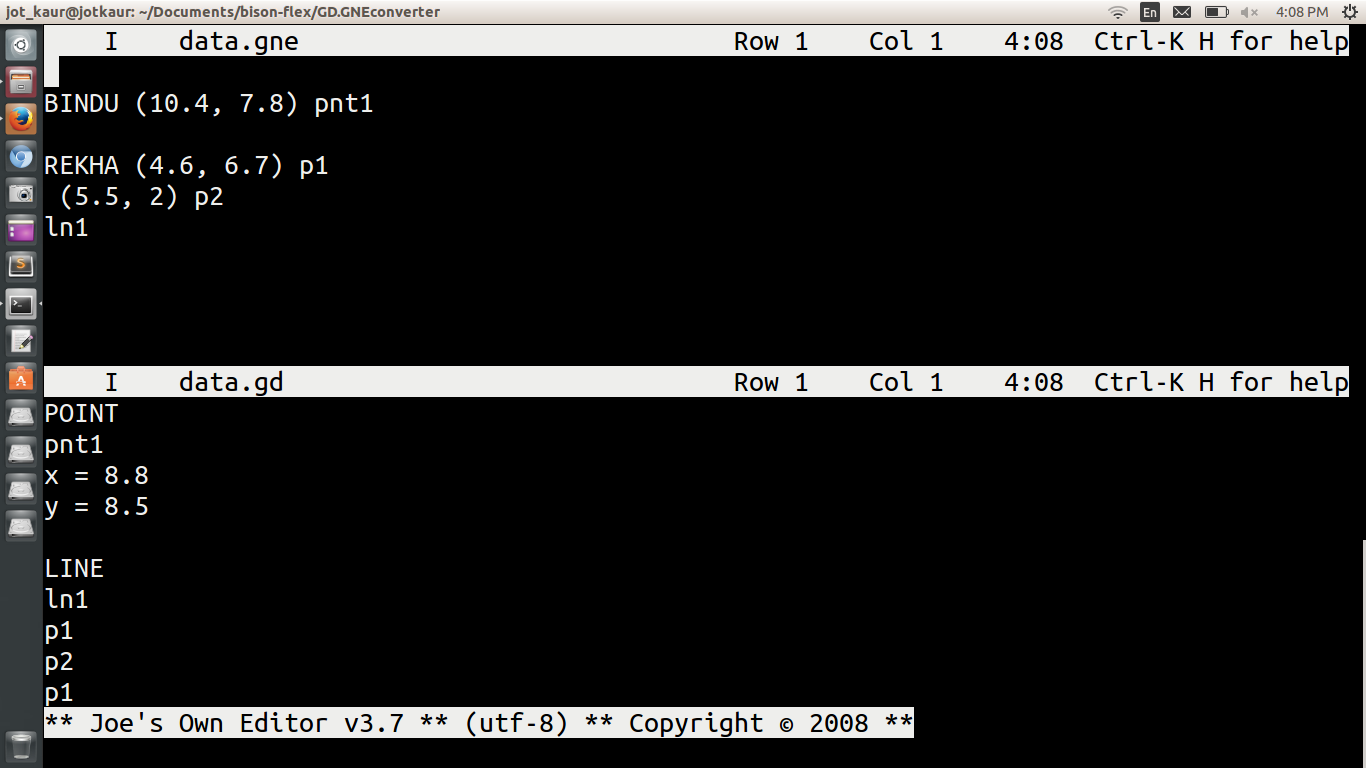
\includegraphics[scale=0.2]{images/gneoutput.png}
\caption{Output files generated by parser}
\end{figure}

\newpage
\subsection{XCAD-ECAD Converter}

\item It asks the user about his requirements regarding the conversion of file formats i.e which file format will be his input file and which one will be his output file. On the basis of his input, the further working of the software is proceeded.
\begin{figure} [h!]
\centering
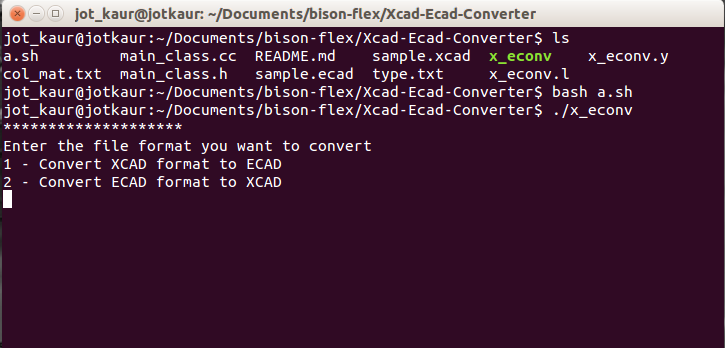
\includegraphics[scale=0.3]{images/ecad2.png}
\caption{List of files that we write}
\end{figure}

\item If the user chooses first option, this window is printed, which guides the user about how he is going to direct the system about his input file in the std format and the output file in the flt format.
\begin{figure} [h!]
\centering
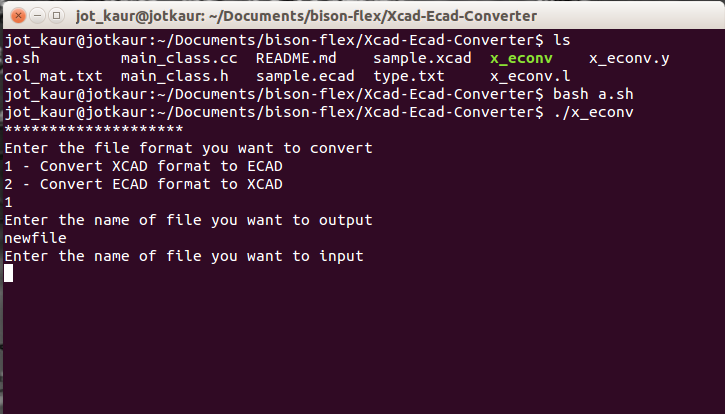
\includegraphics[scale=0.3]{images/ecad3.png}
\caption{Output files generated by parser}
\end{figure}

\item This acknowledges the user about the creation of the new output file i.e flt file in the same directory where he is running his software.\\
\begin{figure} [h!]
\centering
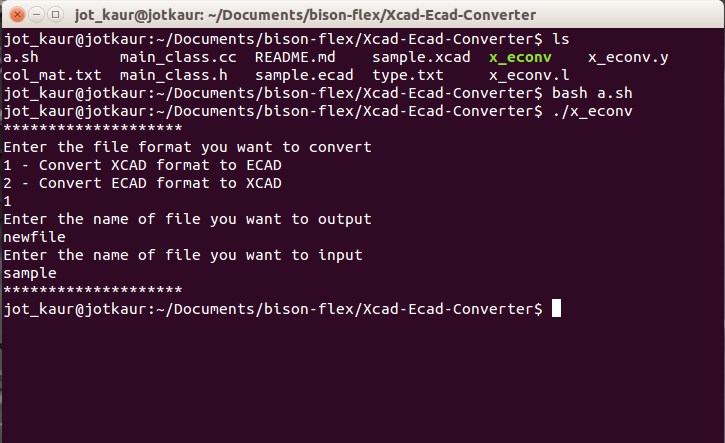
\includegraphics[scale=0.3]{images/ecad4.png}
\caption{Output file}
\end{figure}

\item  It echos a message which acknowledges the user about the creation of the new std file with the name as prescribed by the user, in the same directory in which he is executing the software.
\begin{figure} [h!]
\centering
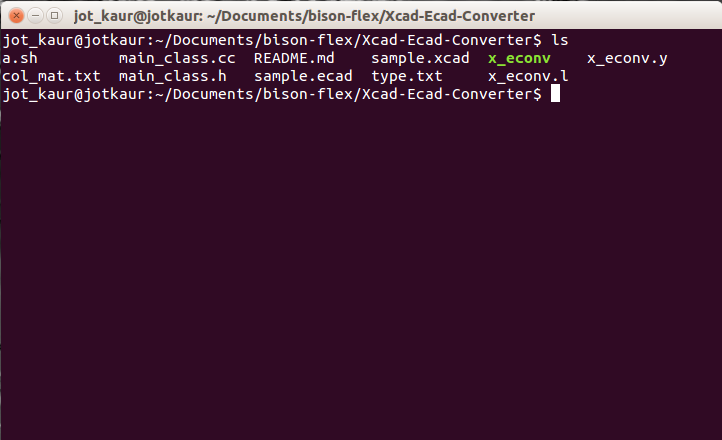
\includegraphics[scale=0.3]{images/ecadfiles.png}
\caption{Execute File}
\end{figure}

\end{enumerate}


\subsection{Felt-Staad-Pro Converter}
snapshots of system with brief detail of each:\\
\begin{enumerate}
\item snapshot 1- It asks the user about his requirements regarding the conversion of file formats i.e which file format will be his input file and which one will be his output file. On the basis of his input, the further working of the software is proceeded.
\begin{figure} [h!]
\centering
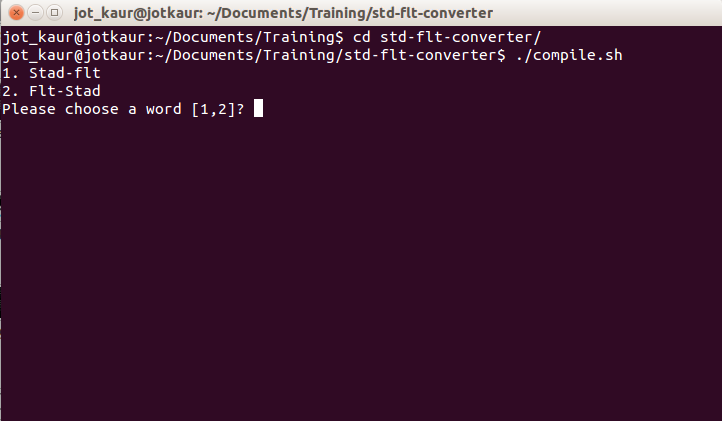
\includegraphics[scale=0.3]{images/1.png}
\caption{File Format }
\end{figure}

\item snapshot 2- If the user chooses first option, this window is printed, which guides the user about how he is going to direct the system about his input file in the std format and the output file in the flt format.
\begin{figure} [h!]
\centering
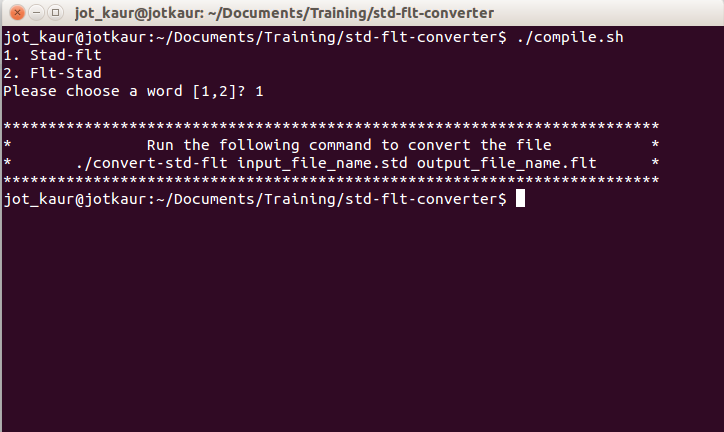
\includegraphics[scale=0.3]{images/2.png}
\caption{Output file}
\end{figure}

\item snapshot 3- This acknowledges the user about the creation of the new output file i.e flt file in the same directory where he is running his software.\\
\begin{figure} [h!]
\centering
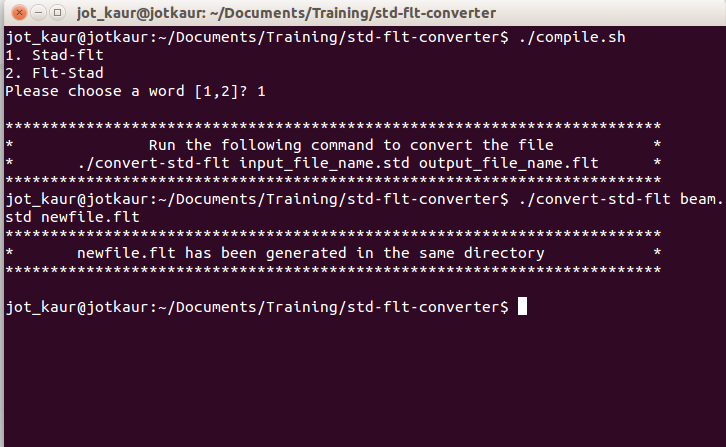
\includegraphics[scale=0.3]{images/3.png}
\caption{Terminal output}
\end{figure}

\item snapshot 4- If the user chooses second option, this message is printed, which lets the user use with the software in a more easier way. A message is displayed which guides the user about the commands he should run to convert his flt file to std file.\\
\begin{figure} [h!]
\centering
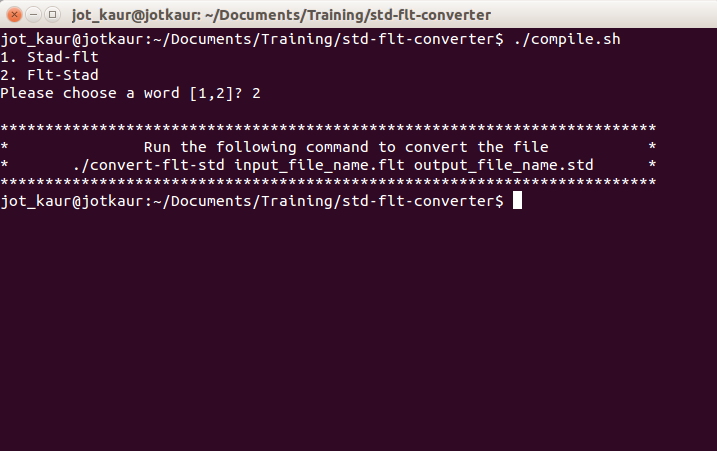
\includegraphics[scale=0.3]{images/5.png}
\caption{Snapshot option file}
\end{figure}

\item snapshot 5- It echos a message which acknowledges the user about the creation of the new std file with the name as prescribed by the user, in the same directory in which he is executing the software.
\begin{figure} [h!]
\centering
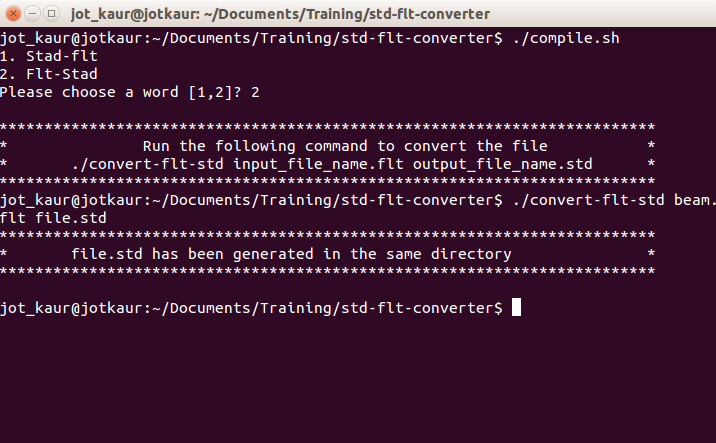
\includegraphics[scale=0.3]{images/6.png}
\caption{Snapshot output file}
\end{figure}


\end{enumerate}


